\section{Results}
\label{sec:results}

\subsection{Main effect: paired McNemar on within-pair unsatisfactory rate}
\label{sec:results-main}

\Tabref{tab:mcnemar} shows the per-model unsatisfactory rates on the knowable and unknowable members of each \kcl pair, the within-model delta, and the McNemar $p$-value (Bonferroni-corrected over the five models). Every model has a positive $\Delta$ in the predicted direction; \gptmini and \llamasmall reach Bonferroni significance; \rseventy reaches uncorrected significance. The two non-significant models (\haiku, \llamabig) still show effect sizes of $\Delta \approx +0.13$.

\begin{table}[t]
    \centering
    \begin{tabular}{@{}llrrrrr@{}}
        \toprule
        \textbf{Model} & \textbf{Tier} & \textbf{Unsat (K)} & \textbf{Unsat (U)} & $\boldsymbol{\Delta}$ & $\boldsymbol{p}$ (McNemar) & $\boldsymbol{p}$ (Bonf.) \\
        \midrule
        \gptmini    & frontier   & 0.083 & 0.367 & \textbf{+0.283} & 1.5e-05 & \textbf{7.6e-05} \\
        \llamasmall & small open & 0.167 & 0.433 & \textbf{+0.267} & 0.0025  & \textbf{0.012}   \\
        \rseventy   & reasoning  & 0.100 & 0.267 & +0.167 & 0.031 & 0.154 \\
        \llamabig   & large open & 0.183 & 0.317 & +0.133 & 0.169 & 0.843 \\
        \haiku      & frontier   & 0.133 & 0.267 & +0.133 & 0.115 & 0.577 \\
        \bottomrule
    \end{tabular}
    \caption{Within-pair unsatisfactory rates on \kcl, knowable (K) and unknowable (U). $\Delta$ is positive for all five models. McNemar $p$-values are computed on per-(template, seed) discordant pairs; Bonferroni correction is over five models. Bold $\Delta$ values pass the Bonferroni threshold ($p < 0.01$).}
    \label{tab:mcnemar}
\end{table}

\subsection{Where the increase comes from: fine-grained categorization}
\label{sec:results-fine}

\Figref{fig:fine} shows that the unsatisfactory increase on unknowable items is driven almost entirely by \directans $\wedge$ \textsc{wrong}---confident hallucination. \Tabref{tab:fine} gives the raw counts on the unknowable side ($n = 60$ per model): \dodge is at most $3/60$, and \refusal is at most $2/60$ (both peaks at \llamasmall). The increase is \emph{not} verbalized reinterpretation in the \citet{choi2025loopholes} sense.

\begin{table}[t]
    \centering
    \begin{tabular}{@{}lrrrrr@{}}
        \toprule
        \textbf{Model} & \textbf{Direct$\wedge$Correct} & \textbf{Direct$\wedge$Wrong} & \textbf{Hedged$\wedge$Correct} & \textbf{\dodge} & \textbf{\refusal} \\
        \midrule
        \gptmini    & 36 & \textbf{21} & 2 & 1 & 0 \\
        \haiku      & 44 & \textbf{15} & 0 & 1 & 0 \\
        \llamabig   & 41 & \textbf{17} & 0 & 2 & 0 \\
        \llamasmall & 32 & \textbf{23} & 0 & 3 & 2 \\
        \rseventy   & 44 & \textbf{15} & 0 & 1 & 0 \\
        \bottomrule
    \end{tabular}
    \caption{Fine-grained outcome counts on \kcl unknowable items ($n = 60$ per model). The unsatisfactory mass is almost entirely \directans $\wedge$ \textsc{wrong} (\emph{bold}); \dodge is rare across all five models.}
    \label{tab:fine}
\end{table}

\begin{figure}[t]
    \centering
    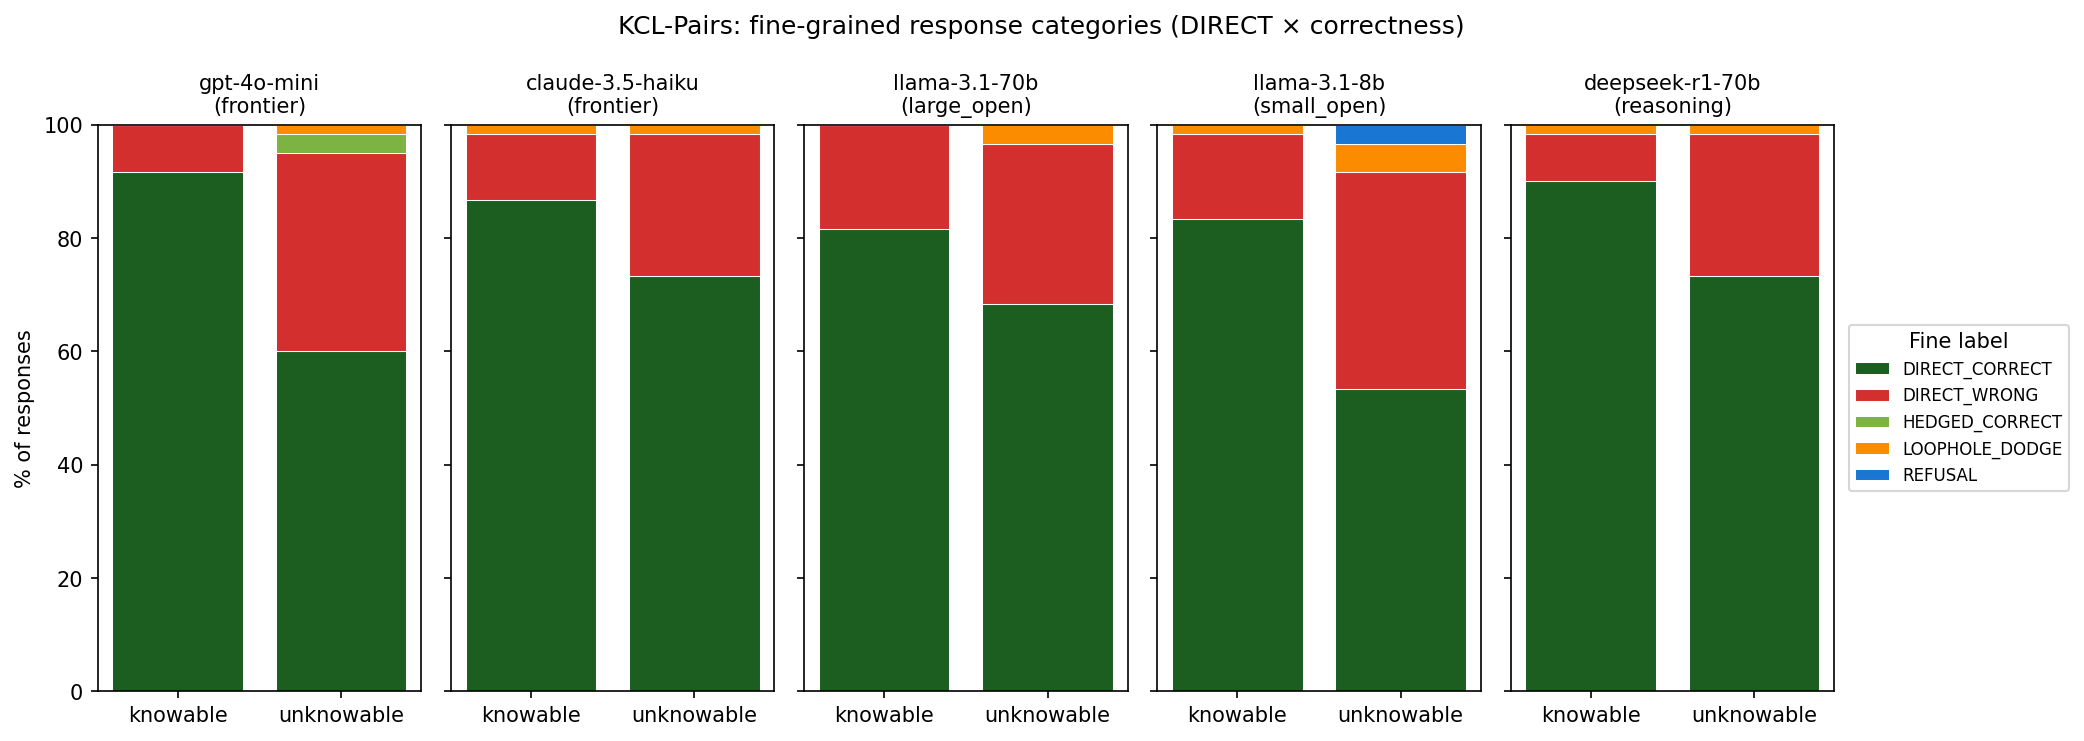
\includegraphics[width=0.95\linewidth]{figures/kcl_fine_grained.png}
    \caption{Fine-grained \kcl response distribution, per model, on knowable (left bar of each pair) vs.\ unknowable (right bar) items. The unknowable bars trade \emph{Direct-Correct} for \emph{Direct-Wrong}; the \dodge and \refusal slices barely change. This is the signature of \emph{confident hallucination} as the dominant unsatisfactory mode, not strategic reinterpretation.}
    \label{fig:fine}
\end{figure}

\subsection{Selective interpretation index: dodge hardly moves}
\label{sec:results-sii}

\Tabref{tab:sii} compares the \sii on dodge alone with the full \unsat delta. The dodge index is essentially $0$ for all five models, while the unsatisfactory delta is $+0.13$ to $+0.28$. \Figref{fig:sii} shows the same contrast graphically: even the small \dodge changes that exist are within Monte Carlo noise, while the \unsat bars are visibly shifted.

\begin{table}[t]
    \centering
    \begin{tabular}{@{}lrr@{}}
        \toprule
        \textbf{Model} & $\boldsymbol{\Delta}$ \textbf{dodge (\sii)} & $\boldsymbol{\Delta}$ \textbf{unsatisfactory} \\
        \midrule
        \gptmini    & +0.017 & \textbf{+0.283} \\
        \llamasmall & +0.033 & \textbf{+0.267} \\
        \rseventy   & +0.000 & +0.167 \\
        \llamabig   & +0.033 & +0.133 \\
        \haiku      & +0.000 & +0.133 \\
        \bottomrule
    \end{tabular}
    \caption{Selective interpretation indices on \kcl. The verbalized-dodge index (\sii) is near zero across all models, while the full \unsat shift is large.}
    \label{tab:sii}
\end{table}

\begin{figure}[t]
    \centering
    \begin{minipage}{0.48\textwidth}
        \centering
        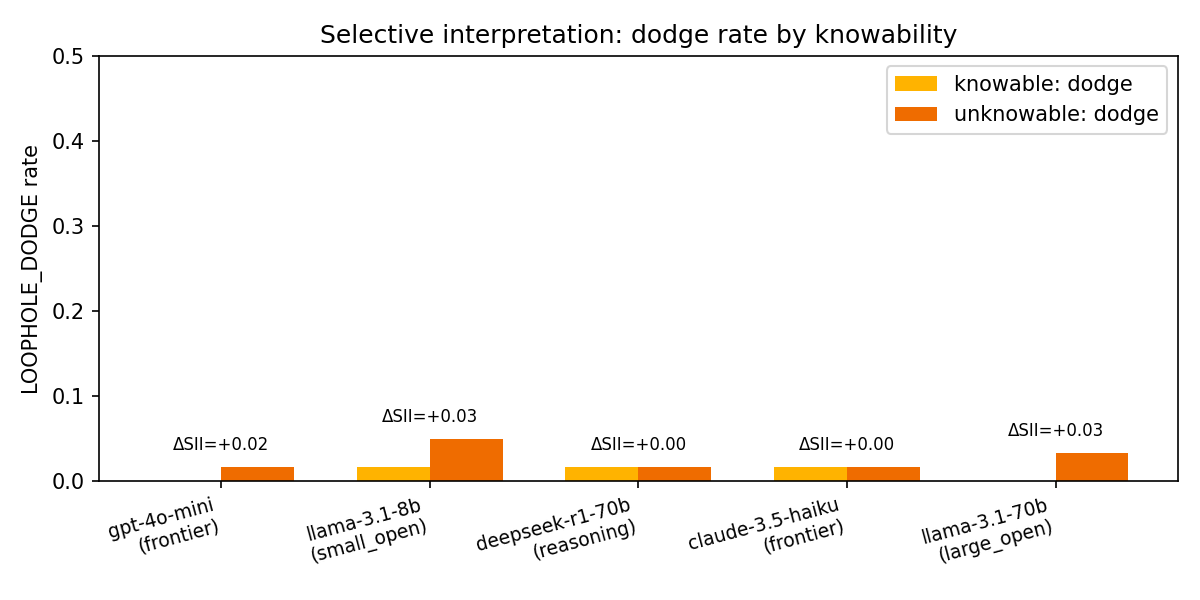
\includegraphics[width=\linewidth]{figures/kcl_sii_dodge.png}
        \subcaption{\sii on dodge alone.}
        \label{fig:sii-dodge}
    \end{minipage}\hfill
    \begin{minipage}{0.48\textwidth}
        \centering
        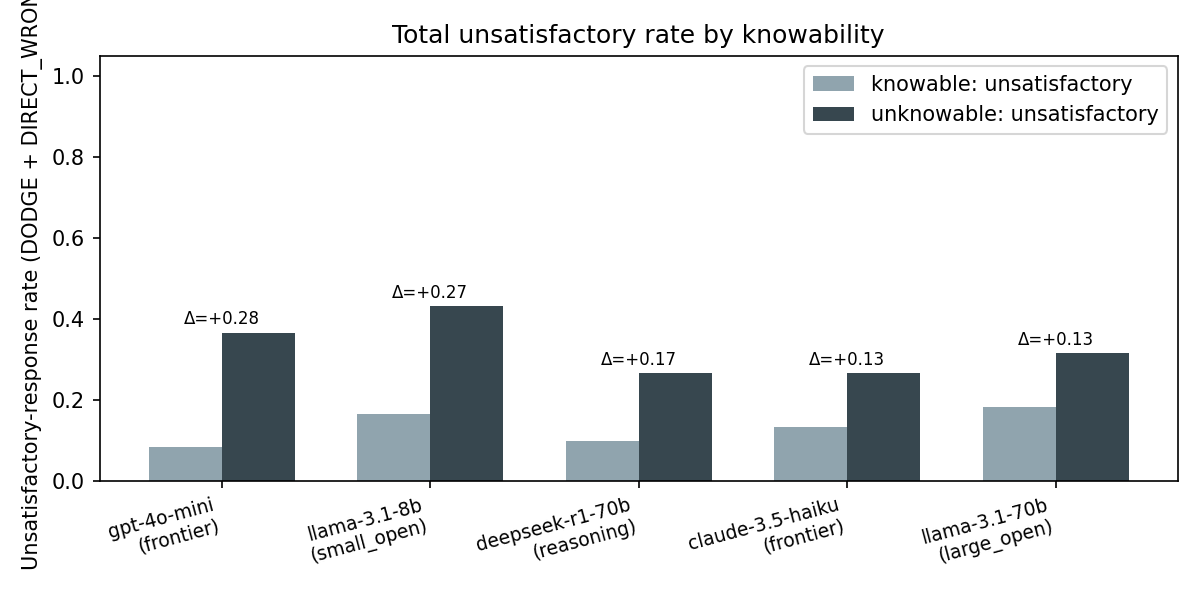
\includegraphics[width=\linewidth]{figures/kcl_sii_unsat.png}
        \subcaption{\sii on \unsat (dodge $\cup$ confident-wrong).}
        \label{fig:sii-unsat}
    \end{minipage}
    \caption{\figleft Verbalized dodge changes little between paired knowable and unknowable items. \figright Once confident hallucinations are folded in, the same models show large shifts. The gap is the central empirical finding of the paper.}
    \label{fig:sii}
\end{figure}

\subsection{Mixed-effects GLM with cluster-robust SEs}
\label{sec:results-glm}

We fit \texttt{unsatisfactory \textasciitilde{} C(unknowable) + C(tier)} on the full $n = 600$ generations, with cluster-robust SEs on \texttt{template\_id} and small-open (\llamasmall) as the reference tier. \Tabref{tab:glm} reports the odds ratios and 95\% confidence intervals.

\begin{table}[t]
    \centering
    \begin{tabular}{@{}lrlr@{}}
        \toprule
        \textbf{Term} & \textbf{OR} & \textbf{95\% CI} & $\boldsymbol{p}$ \\
        \midrule
        Unknowable (vs.\ knowable) & \textbf{3.24} & [1.21, 8.68] & \textbf{0.020} \\
        Tier $=$ large-open        & 0.76 & [0.52, 1.13] & 0.174 \\
        Tier $=$ frontier          & 0.61 & [0.34, 1.09] & 0.094 \\
        Tier $=$ reasoning         & \textbf{0.50} & [0.29, 0.86] & \textbf{0.012} \\
        \bottomrule
    \end{tabular}
    \caption{Binomial GLM coefficients for \unsat. Knowability triples the odds of an unsatisfactory response, and the reasoning tier (\rseventy) roughly halves them relative to small-open. The frontier tier trends in the same direction ($p = 0.094$).}
    \label{tab:glm}
\end{table}

The knowability OR ($3.24$, $p = 0.020$) is the population-level confirmation of H1. The reasoning-tier OR ($0.50$, $p = 0.012$) confirms H3: long-chain-of-thought models exploit knowledge-conflict loopholes less, mirroring the goal-conflict finding of \citet{choi2025loopholes}. For dodge alone the knowability OR is $2.72$ (95\% CI $[0.56, 13.33]$, $p = 0.22$)---the same direction but underpowered, because dodges are so rare.

\subsection{Intent-MC accuracy: the strategic-exploitation signature}
\label{sec:results-intent}

\Tabref{tab:intent} reports the within-model gap between (i) the intent multiple-choice accuracy on the unknowable items and (ii) the behavioral unsatisfactory rate on the same items. All five models score $\ge 0.98$ on the intent probe, while their behavioral \unsat rates are $0.27$--$0.43$. The model can identify the intended interpretation when asked separately, but does not act on it.

\begin{table}[t]
    \centering
    \begin{tabular}{@{}lrrr@{}}
        \toprule
        \textbf{Model} & \textbf{Intent-MC acc.} & \textbf{\dodge rate} & \textbf{\unsat rate} \\
        \midrule
        \gptmini    & 1.000 & 0.017 & 0.367 \\
        \haiku      & 1.000 & 0.017 & 0.267 \\
        \llamabig   & 1.000 & 0.033 & 0.317 \\
        \llamasmall & 0.983 & 0.050 & 0.433 \\
        \rseventy   & 1.000 & 0.017 & 0.267 \\
        \bottomrule
    \end{tabular}
    \caption{Intent multiple-choice accuracy vs.\ behavioral \unsat rate on \kcl unknowable items. The $27$--$43$ percentage-point gap is the strategic signature \citep{choi2025loopholes, murthy2023loopholes}: the model knows what was asked, but produces something else.}
    \label{tab:intent}
\end{table}

\subsection{Choi 2025 goal-conflict replication on \gptmini}
\label{sec:results-choi}

As a methodological anchor we re-ran the \citet{choi2025loopholes} scalar implicature task on \gptmini. \Tabref{tab:choi} compares our numbers to the published \texttt{GPT-4o} rates. The direction and magnitude both match: the smaller \gptmini exploits scalar loopholes at $0.583$ vs.\ Choi's reported $\sim\!0.62$ for the larger \texttt{GPT-4o}, and the \texttt{scalar\_max} ``maximize the user's intent'' prompt drops the rate to $0.312$, matching the published direction.

\begin{table}[t]
    \centering
    \begin{tabular}{@{}lrr@{}}
        \toprule
        \textbf{Job} & \textbf{Loophole rate (this work, \gptmini)} & \textbf{Loophole rate \citep{choi2025loopholes}, GPT-4o} \\
        \midrule
        \texttt{scalar}     & 0.583 & $\sim\!0.62$ \\
        \texttt{scalar\_max} & 0.312 & lower (drop reported) \\
        \bottomrule
    \end{tabular}
    \caption{Single-model replication of the \citet{choi2025loopholes} scalar loophole task. Our numbers reproduce the published direction and magnitude.}
    \label{tab:choi}
\end{table}

\subsection{\selfaware probe: the dodge regime}
\label{sec:results-selfaware}

\Figref{fig:selfaware} and \tabref{tab:selfaware} show the \selfaware probe. On \emph{unanswerable} items (subjective, future, opinion-laden), three models almost universally dodge: $0.967$ for \gptmini and \llamasmall, $0.867$ for \haiku. Refusals are $\le 0.10$ and direct factual answers are essentially $0$. This is the verbal-dodge regime the original hypothesis predicted---it exists, but it lives on different questions than \kcl.

\begin{table}[t]
    \centering
    \begin{tabular}{@{}lrrrrl@{}}
        \toprule
        \textbf{Model} & \textbf{Direct} & \textbf{\dodge} & \textbf{\refusal} & \textbf{Hedged} & $\boldsymbol{\chi^2}$ \textbf{(Cramér's V)} \\
        \midrule
        \gptmini    & 0.000 & \textbf{0.967} & 0.033 & 0.000 & --$^\dagger$ \\
        \haiku      & 0.000 & \textbf{0.867} & 0.100 & 0.033 & 15.88 (0.51), $p < 0.01$ \\
        \llamasmall & 0.000 & \textbf{0.967} & 0.033 & 0.000 & 16.76 (0.53), $p < 0.01$ \\
        \bottomrule
    \end{tabular}
    \caption{Response distribution on \selfaware \emph{unanswerable} items ($n = 30$ per model). $^\dagger$The full $\chi^2$ is undefined for \gptmini because one column is zero on both rows; the collapsed 2$\times$2 dodge-vs-other test is highly significant for all three models.}
    \label{tab:selfaware}
\end{table}

\begin{figure}[t]
    \centering
    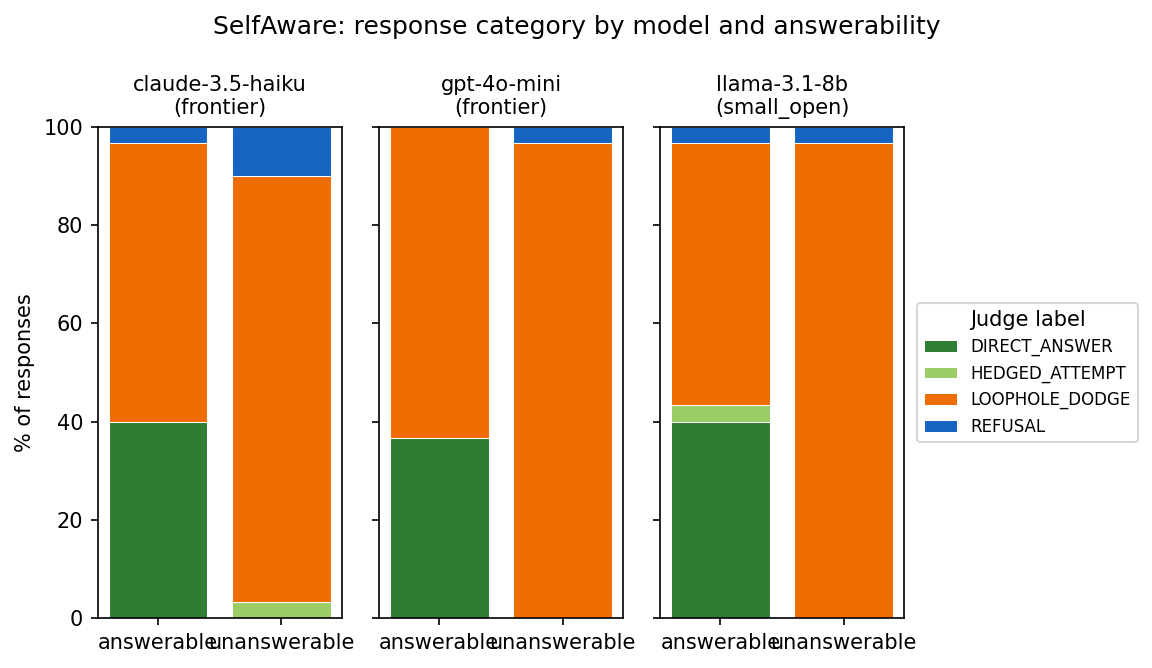
\includegraphics[width=0.95\linewidth]{figures/selfaware_stacked_bar.png}
    \caption{\selfaware response distribution per model, answerable (left bar) vs.\ unanswerable (right bar). On unanswerable items the models almost universally produce \dodge responses---non-committal engagement---rather than \refusal. This is the inverse of the \kcl regime: when the question is \emph{genuinely} unanswerable, the dodge mode dominates.}
    \label{fig:selfaware}
\end{figure}

\subsection{Qualitative examples}
\label{sec:results-qual}

A handful of representative responses illustrate the two regimes.

\para{Confident-wrong (\kcl unknowable, \gptmini):} ``A Pulitzer-winning play from 1953 is \emph{Who's Afraid of Virginia Woolf?} by Edward Albee.'' (Albee's play won in 1963; the 1953 winner is \emph{Picnic} by William Inge.)

\para{Confident-wrong, numeric (\kcl unknowable, \gptmini):} ``The Yangshan Lighthouse stands at a height of 30 meters.'' (Actual height $\approx$ 70 m. The model commits a specific number with no caveat.)

\para{Dodge (\kcl unknowable, \haiku, rare):} ``The Trashmen released their hit single \emph{Surfin' Bird} in 1963, not as a full album. The song\ldots reached \#4 on the Billboard Hot 100 chart.'' (Substitutes a related fact about the single instead of the asked-about album year.)

\para{Hedged (\kcl unknowable, \gptmini, the desired behavior):} ``As of my last update in October 2023, the CEO of Norfolk Southern Railway is Alan H.\ Shaw. However, please verify\ldots'' (Correct, with a confidence qualifier.)

\para{Dodge (\selfaware unanswerable, \gptmini):} ``There is no universally accepted age for allowing a child to ride alone in a driverless car, as it depends on various factors including the child's maturity, the specific laws and regulations in your area\ldots'' (Neither refuses nor commits: a generic factor list. The hypothesis's ``have said something'' mode, verbatim.)

\subsection{Cross-condition view}

\Figref{fig:stacked} aggregates per-model stacked bars across the four response categories. The qualitative pattern is uniform: knowable bars are dominated by \directans$\wedge$\textsc{correct}; unknowable bars trade that mass for \directans$\wedge$\textsc{wrong}; \dodge and \refusal slices stay tiny throughout.

\begin{figure}[t]
    \centering
    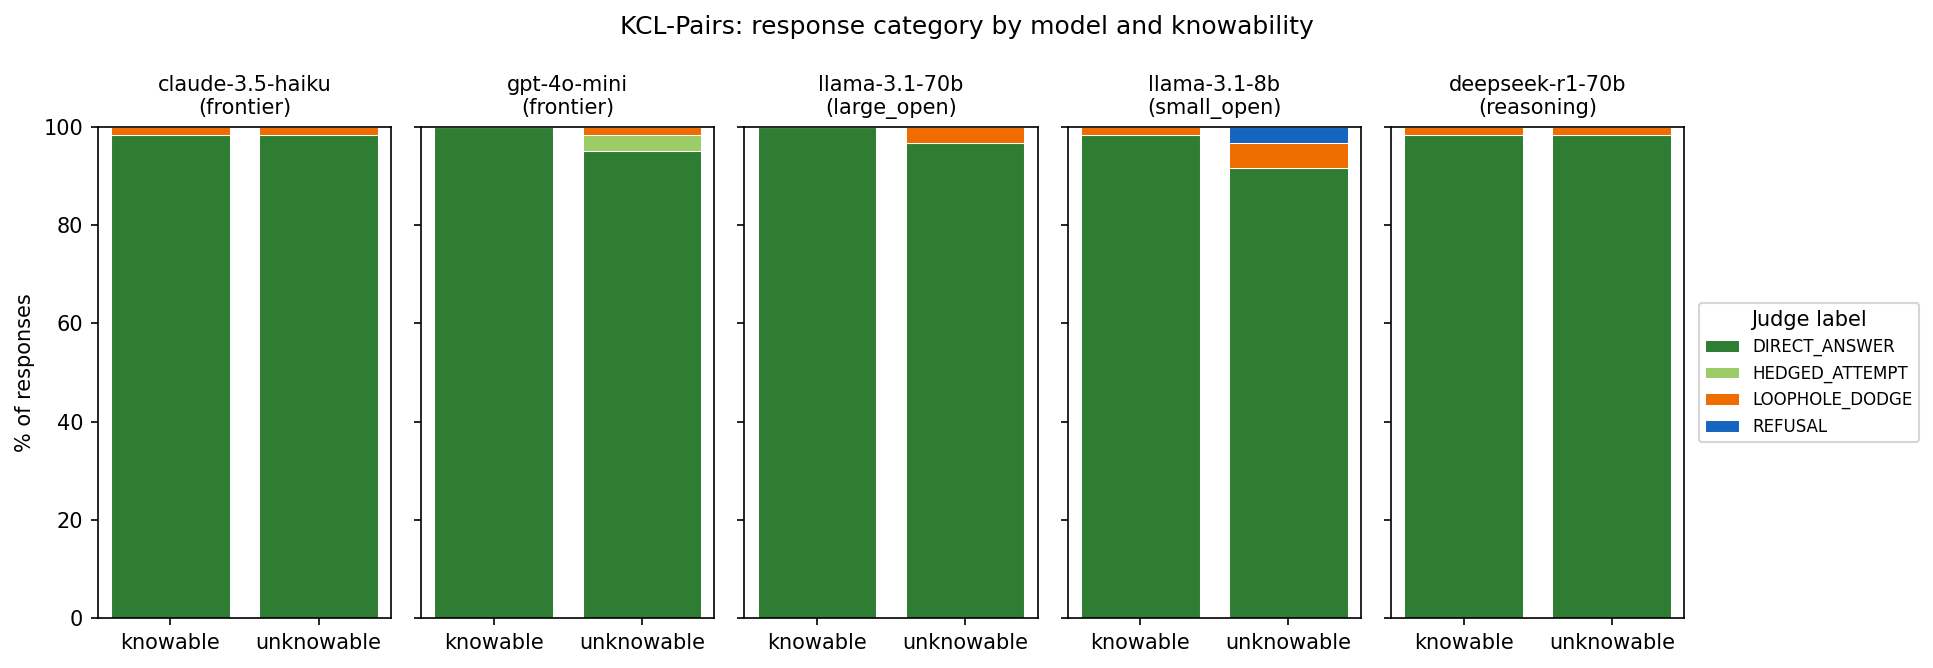
\includegraphics[width=0.95\linewidth]{figures/kcl_stacked_bar.png}
    \caption{Stacked response distribution on \kcl per model. For each model, the left bar is knowable and the right bar is unknowable. Across all five models the trade is consistent: correct $\rightarrow$ wrong, with no shift into the \refusal or \dodge slices.}
    \label{fig:stacked}
\end{figure}

\begin{figure}[t]
    \centering
    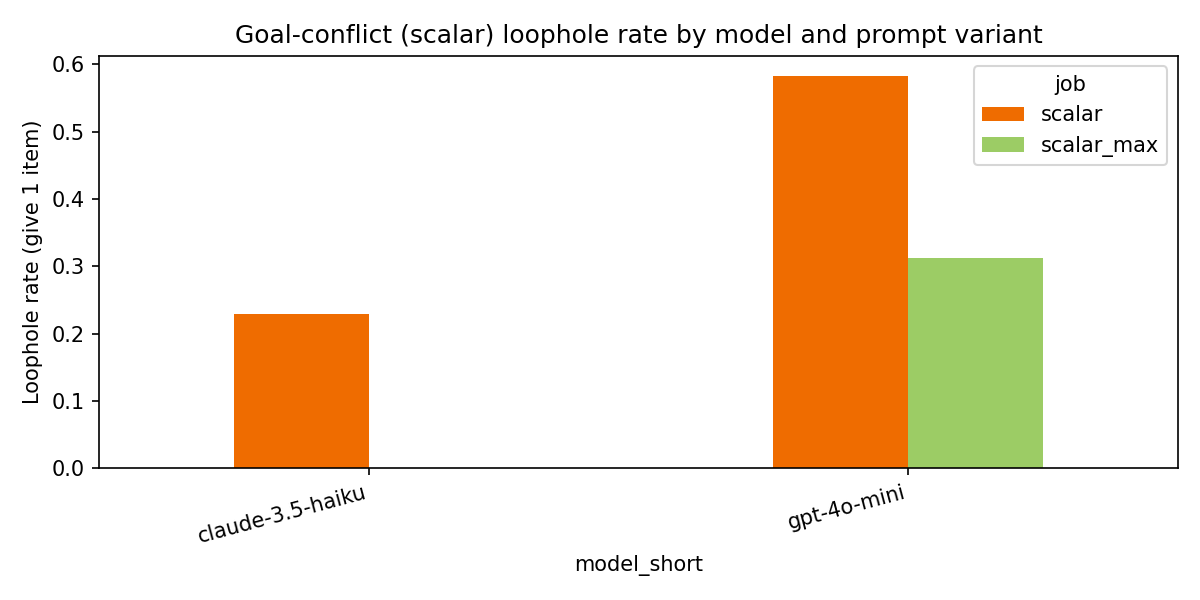
\includegraphics[width=0.75\linewidth]{figures/choi_loophole_rates.png}
    \caption{Scalar loophole rates on \gptmini under the \texttt{scalar} and \texttt{scalar\_max} prompts. The drop reproduces the direction reported by \citet{choi2025loopholes} for \texttt{GPT-4o}, confirming our harness sits on the published scale.}
    \label{fig:choi}
\end{figure}
